\documentclass{article}

\usepackage[final]{corl_2026}
\usepackage{graphicx}
\usepackage{booktabs}
\usepackage{amsmath}
\usepackage{url}

\title{Reward-Shaped Self-Play and Baseline-Focused Fine-Tuning for SoccerTwos}

\author{
  Hanqin Zhang\\
  Georgia Institute of Technology\\
  United States\\
  \texttt{replace1@gatech.edu}
  \And
  Ruihuan Gao\\
  Georgia Institute of Technology\\
  United States\\
  \texttt{replace2@gatech.edu}
}

\begin{document}
\maketitle

\begin{abstract}
We train a competitive SoccerTwos policy with proximal policy optimization (PPO) using Ray RLlib and the Unity ML-Agents simulator. Our main modification is reward shaping: in addition to sparse goal rewards, we add dense incentives for moving the ball toward the opponent goal, reaching the ball sooner, clearing danger near our own goal, and avoiding unnecessary time steps. We first train a reward-shaped shared policy (Agent~2) to obtain a stable warm-start checkpoint, then fine-tune that policy against the course baseline with a frozen-opponent mixture and an archived self-play pool (Agent~4). The final submitted agent is implemented in \texttt{TEAM5\_AGENT/agent.py}, which loads checkpoint \texttt{checkpoint-525}. Local evaluation shows the final checkpoint beats the provided baseline $24/30$ times and the random agent $30/30$ times, while the official Gradescope run reported full wins against both provided opponents.
\end{abstract}

\keywords{multi-agent reinforcement learning, PPO, SoccerTwos}

\section{Overview}
SoccerTwos is difficult because rewards are sparse, control is continuous, and the opponent adapts during training. Our hypothesis was that dense, team-aligned shaping would make early exploration less random, while a later fine-tuning stage against the course baseline would convert that generic competency into a stronger competition policy. We therefore built a two-stage pipeline centered on Agent~2 and Agent~4: Agent~2 learned stable reward-shaped play, and Agent~4 warm-started from that checkpoint and targeted the CEIA baseline directly. A brief Agent~3 self-play experiment informed our design choices, but the final report and submission are mainly about the Agent~2 $\rightarrow$ Agent~4 progression.

\section{Method}
\textbf{Algorithm and library.} We used PPO~\citep{schulman2017ppo} with the PyTorch backend in RLlib~\citep{liang2018rllib} and the Unity SoccerTwos environment from ML-Agents~\citep{juliani2020mlagents}. PPO was a good fit because the environment is continuous-control, multi-agent, and moderately expensive to simulate, so stable on-policy updates were more valuable than replay-heavy off-policy methods.

\textbf{Reward modification.} We did not change the observation interface in the final submitted agent, because keeping the default observation format made the autograder path simpler and reduced failure modes. Instead, we modified rewards in \texttt{reward\_wrappers.py}. The shaped reward adds four dense components on top of the environment reward: (1) ball progress in the $x$ direction toward the opponent goal, (2) improvement in the nearest teammate-to-ball distance, (3) a defensive clear bonus when the ball leaves a danger zone near our own goal, and (4) a small per-step penalty. These terms follow the standard intuition of reward shaping~\citep{ng1999reward}: make good intermediate behavior observable without changing the high-level task.

\textbf{Training pipeline.} Agent~2 was our first successful reward-shaped PPO policy. It used one shared policy for all four players, the same two-layer $[256,256]$ MLP architecture as later runs, and reward shaping throughout training. This checkpoint gave us a policy that could reliably chase the ball, rotate into defensive positions, and play complete matches without obviously degenerate behavior. Agent~4 then warm-started from the Agent~2 checkpoint and trained one policy against a frozen CEIA baseline plus a three-policy self-play pool. The pool was updated every 25 training iterations by shifting the newest policy into \texttt{self\_1}, then moving older snapshots to \texttt{self\_2} and \texttt{self\_3}; this is a lightweight version of self-play population training inspired by iterative self-play systems~\citep{silver2017alphagozero}. We also annealed the shaping multiplier from 1.0 to 0.25 so later updates relied more on match outcome than on auxiliary bonuses.

\textbf{File-to-agent mapping.} The submitted autograder agent is \texttt{TEAM5\_AGENT/agent.py}, which loads \texttt{checkpoint-525}. The reward-shaped warm-start stage is implemented in \texttt{train\_agent2\_reward\_player.py}, and the baseline-targeted fine-tuning stage is implemented in \texttt{train\_agent4\_vs\_baseline.py}. We also implemented \texttt{train\_agent5\_vs\_baseline.py} with safer evaluation port handling and a more aggressive baseline mixture, but cluster quota prevented a full run, so Agent~5 is not part of the submitted result.

\section{Results}
Figure~\ref{fig:curves} shows the two main training signals we used to judge progress. The left panel is an earlier reward-shaped training run that we used as a sanity check before final baseline-focused fine-tuning; it confirmed that dense shaping could move the policy away from extremely poor early behavior and into a stable regime with much better ball pursuit and field positioning. The main result is Agent~4: its evaluation win rate against the baseline was noisy at small sample counts, but the trajectory clearly improved over time, rising from $0.40$--$0.60$ in the first $1.5$M steps to sustained $0.80$--$0.85$ around $3.1$--$4.2$M steps. Agent~2's role in this pipeline was to provide the checkpoint that made this fine-tuning stage possible; without that warm start, we repeatedly observed much less stable startup behavior.

\begin{figure*}[t]
\centering
\begin{minipage}{0.32\textwidth}
  \centering
  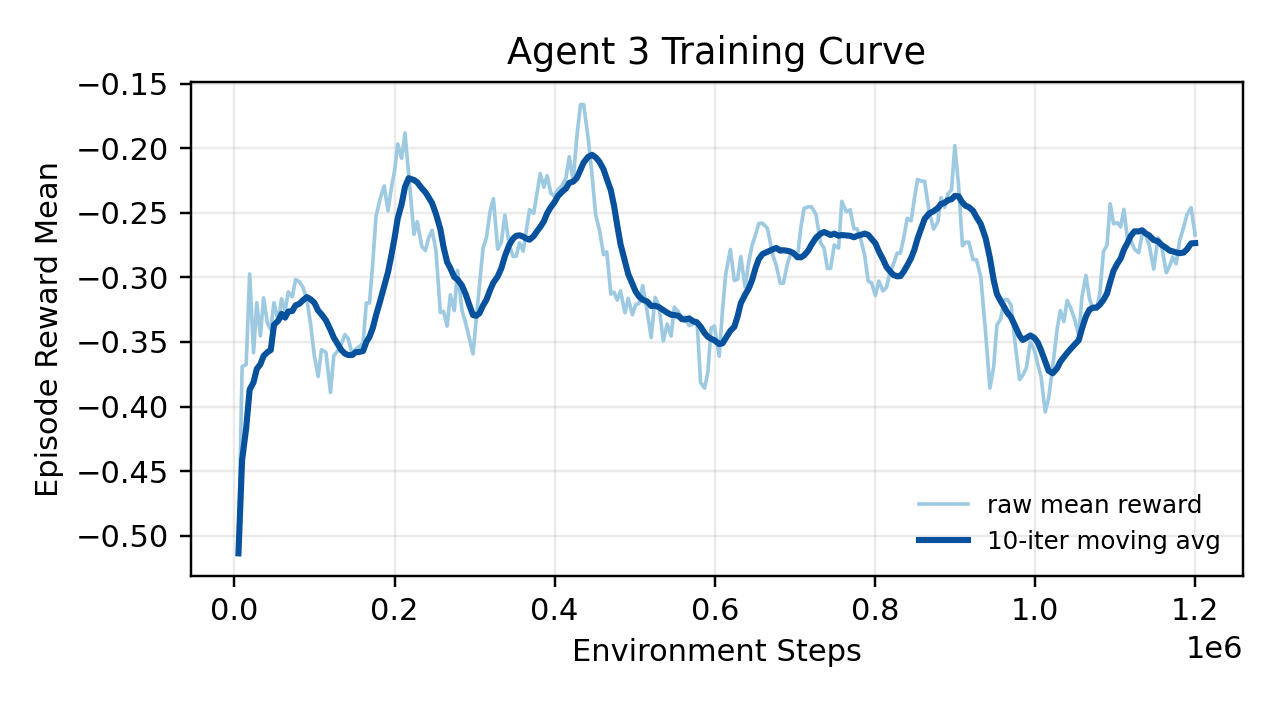
\includegraphics[width=\linewidth]{figures/agent3_training_curve.png}
  \caption*{(a) Preliminary reward-shaped training curve}
\end{minipage}\hfill
\begin{minipage}{0.32\textwidth}
  \centering
  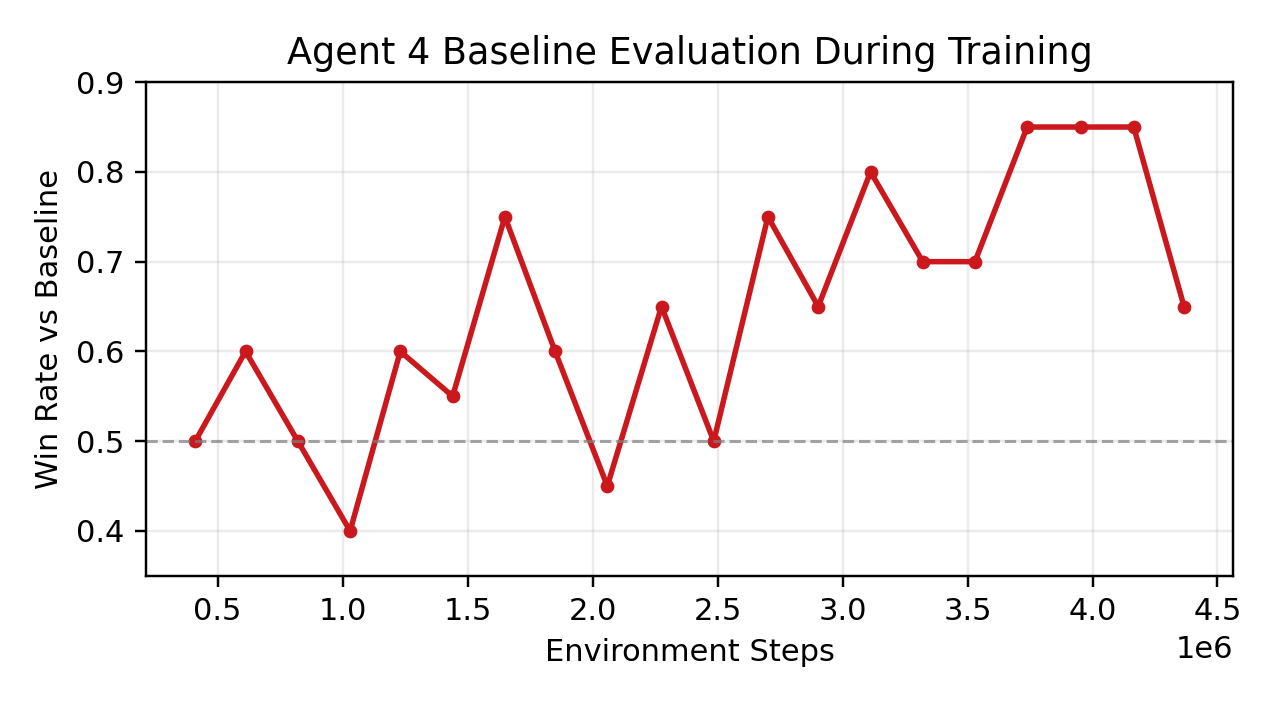
\includegraphics[width=\linewidth]{figures/agent4_baseline_winrate.png}
  \caption*{(b) Agent 4 baseline win rate vs. steps}
\end{minipage}\hfill
\begin{minipage}{0.32\textwidth}
  \centering
  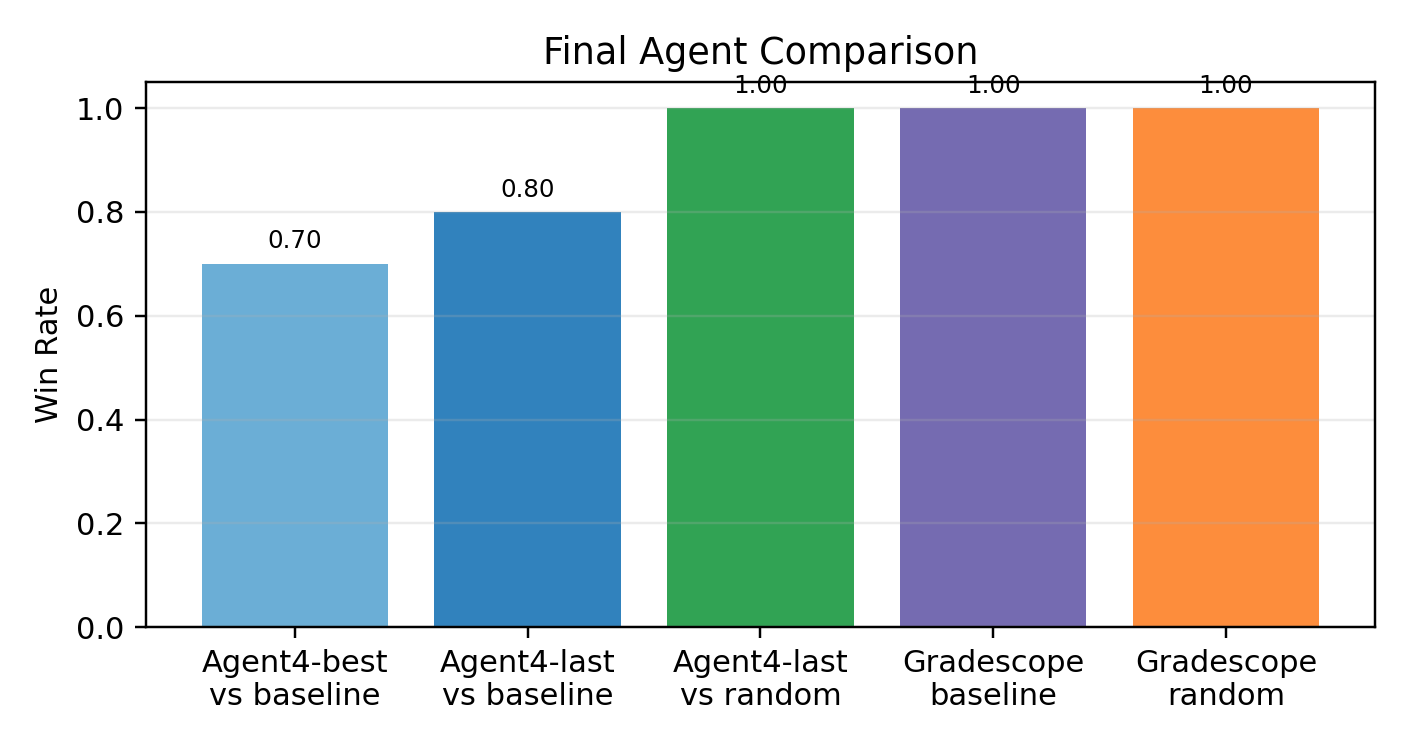
\includegraphics[width=\linewidth]{figures/final_agent_comparison.png}
  \caption*{(c) Final checkpoint comparisons}
\end{minipage}
\caption{Training and evaluation curves for the main stages of our pipeline. Panel (a) is a preliminary reward-shaped run used to validate shaping, panel (b) is the main Agent~4 baseline-targeted learning curve, and panel (c) compares final checkpoint outcomes. Every plotted axis is labeled to match the project rubric: environment steps on the x-axis and either episode reward mean or win rate on the y-axis. The Gradescope bars in panel (c) reflect the official submission outcome reported by the autograder.}
\label{fig:curves}
\end{figure*}

Table~\ref{tab:hparams} lists the exact hyperparameters for the final training run that produced the submitted checkpoint. Figure~\ref{fig:curves}(c) and Table~\ref{tab:eval} compare checkpoints and opponents. On local scripted evaluation, \texttt{checkpoint-450} beat the baseline $21/30$ times, while the later \texttt{checkpoint-525} improved to $24/30$ and also achieved $30/30$ wins against the random agent. The official Gradescope submission reported full wins against both the provided baseline and random agents. This was the policy packaged in \texttt{TEAM5\_AGENT} for submission.

\begin{table}[t]
\centering
\small
\caption{Final training hyperparameters for Agent~4 (\texttt{train\_agent4\_vs\_baseline.py}).}
\label{tab:hparams}
\begin{tabular}{ll}
\toprule
Setting & Value \\
\midrule
Algorithm / library & PPO in RLlib (PyTorch) \\
Initialization & Warm-start from Agent~2 checkpoint \\
Model & 2-layer MLP, $[256,256]$, ReLU, shared value layers \\
Learning rate & $1\times 10^{-4}$ \\
GAE $\lambda$ & $0.95$ \\
Clip parameter & $0.20$ \\
Rollout fragment length & $400$ \\
Train batch size & $8000$ \\
SGD minibatch size & $1024$ \\
SGD epochs per update & $10$ \\
Workers / GPUs in final stable run & $0$ workers, $1$ GPU \\
Opponent mixture & baseline 0.40, self\_1 0.30, self\_2 0.20, self\_3 0.10 \\
Archive / eval interval & every 25 iterations \\
Evaluation episodes & 20 per on-cluster checkpoint test \\
Reward scale schedule & 1.0 $\rightarrow$ 0.25 over 60\% of training \\
\bottomrule
\end{tabular}
\end{table}

\begin{table}[t]
\centering
\small
\caption{Stage summary of the final pipeline.}
\label{tab:stages}
\begin{tabular}{p{0.17\linewidth}p{0.74\linewidth}}
\toprule
Stage & Purpose \\
\midrule
Agent~2 & Train a stable reward-shaped PPO checkpoint that learns ball pursuit, directional play, and defensive recovery. This checkpoint is the warm start for later agents. \\
Preliminary self-play run & Verify that shaping and archived opponents produce non-degenerate learning curves before committing to longer fine-tuning runs. \\
Agent~4 & Fine-tune the warm-start checkpoint directly against the CEIA baseline plus an archived self-play pool. This stage produced the submitted checkpoint \texttt{checkpoint-525}. \\
\bottomrule
\end{tabular}
\end{table}

\begin{table}[t]
\centering
\small
\caption{Performance comparison between discussed checkpoints and official submission outcomes.}
\label{tab:eval}
\begin{tabular}{llll}
\toprule
Policy & Opponent & Episodes & Win rate \\
\midrule
Agent~4 best (\texttt{checkpoint-450}) & CEIA baseline & 30 local & 0.70 \\
Agent~4 final (\texttt{checkpoint-525}) & CEIA baseline & 30 local & 0.80 \\
Agent~4 final (\texttt{checkpoint-525}) & Random agent & 30 local & 1.00 \\
Submitted \texttt{TEAM5\_AGENT} & Gradescope baseline & official & 1.00 \\
Submitted \texttt{TEAM5\_AGENT} & Gradescope random & official & 1.00 \\
\bottomrule
\end{tabular}
\end{table}

\section{Discussion}
The main technical reason the method worked is that shaped rewards gave the policy informative gradients before it could reliably score goals. Agent~2 was important because it turned a sparse-reward competition task into a policy initialization problem: instead of asking Agent~4 to discover basic control and ball pursuit from scratch, we asked it to refine an already competent policy. Ball progress and player-to-ball terms created shorter feedback loops, while the defensive clear bonus encouraged recovery behavior that sparse scoring rewards rarely reinforce early in training. Archived opponents also mattered: self-play alone can overfit to the current policy, but a frozen pool forced the agent to remain robust against older strategies instead of chasing a moving target at every update.

The results were also noisy, which is expected in multi-agent RL. The on-cluster baseline evaluations used only 20 matches per checkpoint, and we observed variance between the best on-cluster checkpoint (\texttt{checkpoint-450}) and the final locally re-evaluated checkpoint (\texttt{checkpoint-525}). Our interpretation is that the difference is mostly evaluation noise plus environment differences between quick local tests and the official autograder. Even with that variance, the trend is consistent: Agent~2 supplied a strong warm start, and targeted Agent~4 fine-tuning against the course baseline pushed the final policy to the strongest submission we obtained.

\section{Conclusion}
Our final SoccerTwos agent combined PPO, dense reward shaping, an Agent~2 warm-start checkpoint, archived self-play, and a baseline-focused Agent~4 fine-tuning stage. The method improved both training stability and downstream win rate, culminating in a submitted agent that passed the official Gradescope random and baseline evaluations. The clearest lesson from this project is that in adversarial continuous-control tasks, shaping and opponent selection matter as much as the optimizer itself: learning a good game requires both useful intermediate rewards and the right distribution of opponents.

\clearpage
\acknowledgments{Replace this line with any acknowledgments you want to include, or leave it empty for the final report.}

\bibliography{project_report}

\end{document}
